\documentclass{article}
\usepackage[utf8]{inputenc}
\usepackage{natbib}
\usepackage{graphicx}
\usepackage{lastpage}
\usepackage{xcolor}
\usepackage{lipsum}
\usepackage[T1]{fontenc}
\usepackage{fancyhdr}
\usepackage{geometry}
\usepackage{url}
\usepackage[dutch]{babel}

\bibliographystyle{abbrv} %abbrvnat geeft problemen

\title{Software Design Document}
\author{} %leave empty
\date{19 november 2014} %ok, manuele datum

\addtolength{\footskip}{1.3cm} % make more space for the footer
\pagestyle{fancyplain} % use fancy for all pages except chapter start
\lhead{}
\cfoot{
\includegraphics[height=1.3cm]{Small_Logo.png}} % right logo
\rfoot{\thepage}
\renewcommand{\headrulewidth}{0.3pt} % remove rule below header
\renewcommand{\footrulewidth}{0.3pt} % remove rule below header
\newcommand{\myparagraph}[1]{\paragraph{#1}\mbox{}\\}

\begin{document}

\makeatletter
\begin{titlepage}

\newcommand{\HRule}{\rule{\linewidth}{0.7mm}} % Defines a new command for the horizontal lines, change thickness here


\vspace*{1.2mm}

\center 

\includegraphics[scale=0.6]{Logo.png}\\[1cm] 
%---------------------------------------------------------------------------------------
%	HEADINGS SECTION
%----------------------------------------------------------------------------------------

\textsc{\LARGE Vrije Universiteit Brussel}\\[0.3cm] % Name of your university/college
\textsc{\large WE-DINF-6537}\\
\textsc{\large Project Software Engineering}\\
\textsc{\large Academiejaar 2014-2015}\\[0.3cm] 
%\textsc{\large Software Engineering}\\[0.7cm] % Major heading such as course name

%----------------------------------------------------------------------------------------
%	TITLE SECTION
%----------------------------------------------------------------------------------------

\HRule \\[0.4cm]
{ \huge \bfseries \@title \\[0.5cm] }
\HRule \\[0.5cm]
 
%----------------------------------------------------------------------------------------
%	AUTHOR SECTION
%----------------------------------------------------------------------------------------

\Large
% laat voorlopig nog even de namen/mailadressen op deze pagina staan
% eerst moeten we zien of er een beter alternatief is om de lege plek dan op te vullen
% anders laten we ze gewoon staan...

%volgens mij ziet het er zo heel goed uit, maar als ze echt wegmoeten mss vub logo groter maken? 
% => OK, ik vind het ook veter zo, we laten ze staan!
Douglas Horemans \textit{<dhoreman@vub.ac.be>}\\
Hannah Pinson \textit{<hpinson@vub.ac.be>}\\
Ivo Vervlimmeren \textit{<ivervlim@vub.ac.be>}\\
Noah Van Es \textit{<noahves@vub.ac.be>}\\
Pieter Steyaert \textit{<psteyaer@vub.ac.be>}\\

\vspace{0.6cm}


\includegraphics[scale=0.4]{VUB_schild.pdf}\\[0.5cm]

{\large 19 november 2014}
\vfill % Fill the rest of the page with whitespace

\end{titlepage}

\newpage
\section*{Versiegeschiedenis}
\addcontentsline{toc}{section}{Versiegeschiedenis}

\begin{center}
\begin{tabular}[t]{| c | c | c | c |}
    \hline
    \textbf{Versie} & \textbf{Datum} & \textbf{Auteurs\cite{note:author}} & \textbf{Beschrijving} \\
    \hline
    
    1.0     &  19/11/2014   &   \begin{tabular}{c} 
                                    Douglas Horemans \\
                                \end{tabular} & Eerste versie \\
    \hline
    2.0     &  15/12/2014   &   \begin{tabular}{c} 
                                    Douglas Horemans \\
                                \end{tabular} & tweede versie \\
    \hline
\end{tabular}
\end{center}
\newpage



\tableofcontents
\newpage

\section{Introductie}

\subsection{Doel}

Dit document beschrijft de architectuur van de software achter SKRIBL. 
Het analyseert het ontwerp en haar (sub)compomenten en geeft een beschrijving
van de werking van het systeem. Op die manier geeft het dus de nodige richtlijnen
voor de implementatie en wordt de filosofie achter het design toegelicht.
Daarnaast geeft het ook aan hoe gebruikers het systeem kunnen gebruiken, zowel
via de grafische webinterface als via een aparte API voor third-parties.

\subsection{Scope}

SKRIBL is een webapplicatie dat gebruikers toelaat om publicaties met elkaar te delen
en te beheren op een interactieve manier. De bedoeling is dus dat men zowel eigen publicaties kan uploaden, alsook op zoek kan gaan naar andere publicaties en zo dus een volledig netwerk kan opbouwen binnen zijn/haar onderzoeksdomein. Het systeem moet hiervoor ook de nodige interface en visualisaties aanbieden, zowel in normale desktop-browsers als voor mobiele apparaten.

Hiervoor zal de software worden uitgerust met een databank en de nodige applicatielogica om aan alle software eisen te voldoen. Ook moet het systeem rekening houden met de webarchitectuur en bekijken hoe de modules en verantwoordelijkheden worden verdeeld onder de client en de server. Voor een volledig overzicht van de beoogde functionaliteit wordt verwezen naar het SRS \cite{Xtreport:SRS}.

\subsection{Overzicht}

Eerst en vooral wordt er in dit document gekeken naar de globale structuur van de software. Hierbij wordt het systeem eerst in grote lijnen besproken, waarna elk onderdeel vervolgens meer in detail wordt bekeken. Daarnaast wordt ook kort de filosofie van het ontwerp toegelicht. 
Vervolgens wordt er gekeken naar de organisatie van de informatie binnen het systeem. Hierbij worden onder andere een schema van de database en diagrammen meegegeven om aan te geven welke data hoe wordt opgeslagen en gebruikt. 
Daarna wordt op een systematische manier bekeken wat elk component binnen het systeem doet. Concreet wordt hier bijvoorbeeld aangegeven hoe een bepaalde methode of algoritme precies werkt.

Nadien volgt een beschrijving van de interfaces, zowel van de grafische webomgeving als van de API. In dit gedeelte kan men terugvinden hoe het systeem gebruikt kan worden en wordt het verloop van de mogelijke handelingen beschreven. Deze handelingen zijn voornamelijk gebaseerd op de requirements zoals opgesteld in het SRS~\cite{Xtreport:SRS}. \\

Dit opmaak van dit document is gebaseerd op de IEEE 1016-1998 standaard voor SDD's\citep{website:IEEE}.

\subsection{Referentiemateriaal}
\begingroup
\renewcommand{\section}[2]{}  % verwijdert titel sectie referenties
\bibliography{referenties}
\endgroup
 
\subsection{Definities en Acroniemen}

\begin{description}

\item[SRS] Software Requirements Specification
\item[SPMP] Software Project Management Plan
\item[SDD] Software Design Document
\item[MVC] Model-View-Controller
\item[API] Application Programming Interface
\item[GUI] Graphical User Interface
\item[SPA] Single-Page Application
\item[JSON] JavaScript Object Notation
\item[AJAX] Asynchronous Javascript and XML
\item[DMBS] Database Management System
\item[(E)ER] (Extended) Entity-Relation
\item[SQL] Structured Query Language
\item[REST] Representational State Transfer
\item[HTML] Hypertext Markup Language
\item[HTTP] Hypertext Transfer Protocol
\item[SSL] Secure Sockets Layer
\item[CSS] Cascading Style Sheets
\item[JS] Javascript

\end{description}

\clearpage

\section{System Overview} %titel in het nederlands?

\subsection{Context}

De software zal uiteindelijk worden geleverd in de de vorm van een webapplicatie. Dit houdt in dat op de server een HTTP(S)-server zal draaien en de client vanuit de browser hiernaar requests zal sturen via een aangename webinterface (zowel voor mobiele als voor desktop-clients).

\subsection{Organisatie}

De software zal worden ontwikkeld volgens de principes van het Agile Development Proces. Zo zal de implementatie van de componenten die in dit document worden beschreven verlopen in verschillende iteraties en sprints. Voor een gedetailleerde beschrijving en planning van deze sprints wordt verwezen naar het SPMP \cite{Xtreport:SPMP}.

\subsection{Gebruikte technologie\"en}

Om het systeem te ontwikkelen wordt gebruik gemaakt van een zuivere \textbf{`HTML/CSS/JS'}-stack.
Daarnaast zullen ook volgende open-source frameworks en libraries worden gebruikt:

\begin{itemize}

\item \textbf{ExpressJS} zal worden gebruikt als framework om de webapplicatie te ontwikkelen om zo gemakkelijker een API voor de server te kunnen ontwerpen\cite{website:ExpressJS}. 

\item \textbf{OrientDB} zal dan weer gebruikt worden als DMBS\cite{website:OrientDB}. OrientDB is een zogeheten NoSQL-database, waarbij data niet wordt georangiseerd in tabellen zoals in een coventionele SQL-database. Specifiek zal gebruik worden gemaakt van de GraphDB-abstractie die OrientDB aanbiedt bovenop hun standaard database. 
Dit laat toe om om alle informatie rondom gebruikers, publicaties, ... in SKRIBL te modelleren als een graaf. (voor de communicatie over het binary protocol wordt gebruik gemaakt van oriento \cite{website:Oriento}) 

\item \textbf{Swagger} zal gebruikt worden om de RESTFul API te documenteren naar 3rd-parties toe\cite{website:Swagger}. Swagger kan tevens ge\"integreerd worden met Express om gemakkelijker deze documentatie te genereren. 

\item \textbf{AJAX} zal op de client worden gebruikt om op een asynchrone (en dus gebruiksvriendelijke) manier requests te sturen naar de server en vervolgens de UI te updaten. Deze technologie is van cruciaal belang om te voldoen aan de design filosofie die wordt beschreven in \ref{sec:rationale}.

\item Daarnaast zal voor de front-end gebruik worden gemaakt van \textbf{AngularJS}. AngularJS  is een zeer flexibel MVC-framework dat HTML uitbreidt met specifieke directives, controllers, ... \cite{website:AngularJS}. 
\end{itemize}

Ten slotte zal de server als onderliggende (open-source) runtime gebruik maken van \textbf{NodeJS}. NodeJS maakt het mogelijk om ook server-side Javascript te gebruiken met een performant event-driven (m.a.w. asynchroon, non-blocking) model\cite{website:NodeJS}. 

\section{System Architecture}

\subsection{Design Rationale}
\label{sec:rationale}

Deze sectie bespreekt eerst de algemene filosofie en structuur achter het ontwerp. Veel van deze principes zijn gebaseerd op het concept van `Web 2.0'-applicaties.
Er is gekozen om gebruik te maken van een MVC-structuur om de applicatielogica (`model') en de UI (`view') gescheiden te houden. 
Hieronder vindt men een grafische voorstelling van dit concept:

\begin{figure}[!h]
\centering
 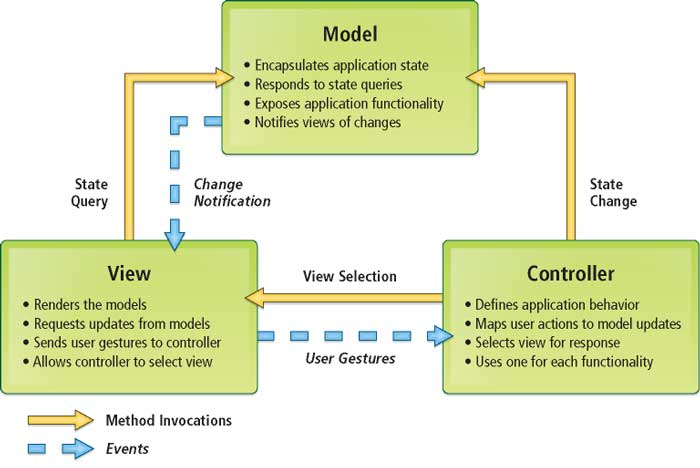
\includegraphics[width=140mm]{MVC.jpg}
 \caption{Illustratie van het MVC-patroon}
 \label{Model-View-Controller}
\end{figure}

\thispagestyle{fancy}
Hierbij zal de webserver voornamelijk de rol van M op zich nemen, terwijl de client de VC-rollen zelf zal beheren. We kunnen hier dus niet langer spreken over een thin, maar wel over een Rich client (rich betekent hier niet noodzakelijk `fat'; onder model wordt ook de applicatielogica rondom dit model verstaan, waardoor de server nog altijd deze belangrijke functies zal moeten implementeren).

Op die manier zal de applicatie in feite het concept van een Single-Page Application (SPA) volgen, waarbij alle functionaliteit van de server wordt vrijgegeven via een RESTFul API. Hierdoor wordt het gemakkelijker om later aparte desktop en mobiele versies aan te maken en kunnen ook andere developers gebruik maken van SKRIBL.

\subsection{Architectuur}

Op basis van deze filosofie kan men de architectuur indelen in een three-tier model met een client tier, server tier, en database tier. Op de client tier gebeurt alle user-interactie met de view en wordt de front-end applicatie beheert via controllers. Deze zullen de nodige gegevens halen via de (RESTful) API van de server, die ook de voornaamste services aan de front-end zal leveren. Voor de uiteindelijke interactie met de data zelf, zal deze server-tier dan ten slotte ook communiceren met de database-tier, waarop de OrientDB-database zich bevindt. \\
Hieronder vindt men een visualisatie van deze architectuur:

\begin{figure}[!h]
\centering
 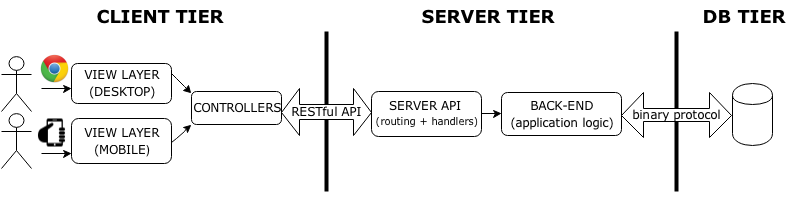
\includegraphics[width=140mm]{Architecture.png}
 \caption{Verschillende tiers in de webapplicatie}
 \label{Architecture}
\end{figure}

\subsection{Decompositie}

Dit onderdeel geeft een beknopt overzicht van de verschillende onderdelen uit bovenstaande architectuur. Voor een gedetailleerde beschrijving van hun individuele componenten wordt verwezen naar sectie~\ref{sec:components}.

\subsubsection{Client Tier}

\paragraph{Views} 
De views vormen hier de GUI voor de eindgebruiker en verschillen voor desktop en mobiele gebruikers. Om het concept van de Single-Page Application te verwezenlijken, zal de server daarom bij bezoek van de website een zogeheten template aanleveren, afhankelijk van het apparaattype van de gebruiker.
Deze template zal gebruik maken van AngularJS en voldoende applicatielogica bevatten (in JavaScript) om tijdens het verloop van de applicatie zelf de interface te laten evolueren.

\paragraph{Controllers} 
De controllers zullen via de AngularJS-directive `ng-controller' worden verbonden aan de views en handelingen van de gebruiker verwerken. Meestal houdt dit in dat een AJAX-call naar de server zal worden gemaakt en het resultaat (meestal in JSON-formaat) geparsed en gebruikt zal worden om zo de view te updaten.

\subsubsection{Server Tier}

\paragraph{Server API} 
Dit gedeelte van de Server API is verantwoordelijk voor het afhandelen van requests van de client. Afhankelijk van het type request en de route (path) zal een bepaalde handler worden opgeroepen die gebruik zal maken van de back-end om de bijhorende applicatielogica uit te voeren en het juiste resultaat naar de client terug te sturen. Als ingangspunt van de server-tier is dit gedeelte dus ook verantwoordelijk voor het opstellen van de RESTful API.

\paragraph{Back-end} 
De back-end voorziet dan weer de meeste functionaliteit van de applicatie. Het interageert met het model via de database-tier en bestaat uit verschillende componenten (en hun bijhorende abstracties) om de `core' van de server-tier te implementeren.

\subsubsection{Database Tier}

Ten slotte zal op de database-tier een server worden opgezet met een database door OrientDB. Het volstaat hier om gewoon via de command-line een meegeleverd shell-script uit te voeren om deze server op te starten.
Een gedetailleerde beschrijving van het ontwerp van deze database volgt in de volgende sectie. 

\clearpage

\section{Data design}

De organisatie van data is cruciaal bij het ontwerp van SKRIBL. Een effici\"ente en persistente datastructuur is nodig om alle relaties tussen de verschillende entiteiten (gebruikers, publicaties, onderzoeksdomeinen, ...) in de applicatie te kunnen modelleren. \\

Om die reden werd gekozen om gebruik te maken van een graph-database. Een graf is veruit de meest natuurlijke representatie van het model en maakt het later ook gemakkelijk om verbanden in de applicatie te verwerken en te visualiseren. 

Concreet werd er gekozen voor OrientDB omdat deze bovenop haar NoSQL-database ook een abstractie aanbiedt die specifiek is ontworpen om graph-databases in elkaar te steken. Daarnaast is het ook een zeer performante DBMS met een zeer gebruiksvriendelijke API. \\

Wat volgt is een (E)ER-model van de huidige structuur in de database:

\begin{figure}[!h]
\centering
 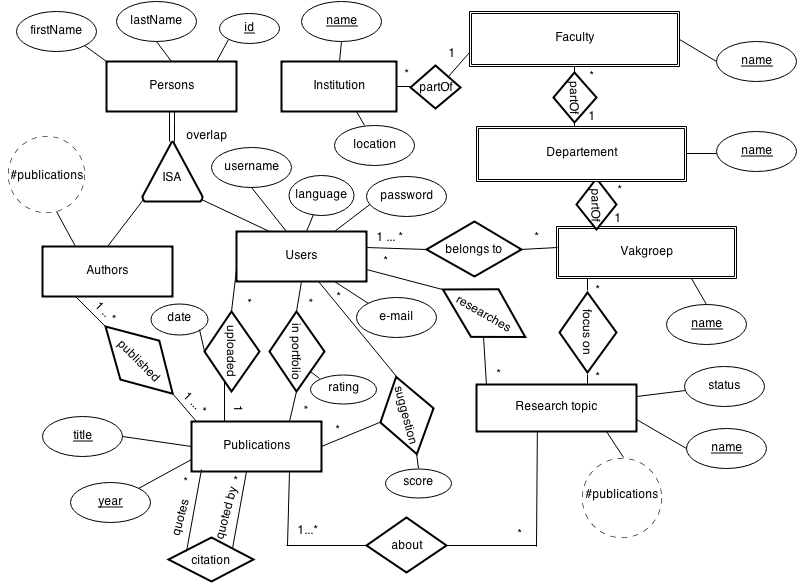
\includegraphics[width=150mm]{ER-model.png}
 \caption{Structuur van de graf in een (E)ER-model}
 \label{ER-model}
\end{figure}

\textit{[In verdere iteraties zal de entiteit publicatie verder gespecialiseerd in verschillende types en zullen er ook meer attributen en entiteiten (conferenties, journals, ...) bijkomen]}

\clearpage

\section{Component Design}
\label{sec:components}

In dit gedeelte worden de verschillende componenten die samen de applicatie vormen, verder toegelicht. Voor triviale componenten wordt enkel een korte beschrijving gegeven, maar indien nodig kan hier ook een volledige specificatie worden uitgewerkt. \\

\textit{[Momenteel zijn het aantal componenten en hun interacties vrij beperkt, later kunnen hier indien nodig eerst hun interfaces en relaties worden ge\"illustreerd in een klassediagram]}

\subsection{Server}

De server zelf vormt het ingangspunt van de server-tier. Deze module kan geconfigureerd worden met bepaalde routes en zal zo de request naar een bepaalde handler delegeren (met de bedoeling om zo een RESTFul API samen te stellen). De handlers zullen op hun beurt dan weer gebruik maken van de back-end, waar de meeste applicatielogica van de server-tier zich bevindt en waar ook de communicatie met de DB-tier plaatsvindt. \\

Momenteel bevat dit component vooral methodes om de server te configureren (port, routes, ...) en om ze te laten opstarten.

\subsection{Routes}

Routes zullen op de server worden gebruikt om de verschillende requests af te handelen.Op die manier wordt het configureren van de Server API gebruiksvriendelijker en overzichtelijker in de code. \\

Een bepaalde route wordt gekenmerkt door een bepaald path (zoals /users) en verschillende handlers voor zowel GET, POST, PUT \& DELETE requests op die route. Een handler is hierbij een functie die een request en response als argumenten nemen en het response-object correct configureert op basis van de request. Een route-object ondersteunt dan getters \textit{get()}, \textit{post()}, ... om deze handlers te gebruiken. 

\subsection{Validation}

Deze module wordt in feite niet alleen op de back-end, maar ook op de front-end gebruikt om input van de gebruiker te valideren. Server-side validation is niet alleen aangewezen vanuit een design-standpunt, maar is ook noodzakelijk om veiligheidsredenen. Client-side validation zorgt dan weer voor een aangenamere en effici\"entere gebruikerservaring. \\

Concreet gaat hier in deze module vooral om functies die worden gebruikt om de geldigheid van een gebruikersnaam, wachtwoord, e-mailadres etc. te controleren. Zo zal men in deze module procedures zoals \textit{validUsername(username)}, \textit{validPassword(pwd)}, ... terugvinden.

\subsection{UserInfo}

Deze klasse bevat alle noodzakelijke informatie over een bepaalde gebruiker in het systeem. Zo'n gebruikersinformatie kan ofwel worden geladen uit de database, ofwel kan via een constructor een nieuwe gebruiker worden aangemaakt (bijvoorbeeld bij de registratie). 

Veel van de ge\"exporteerde methodes in deze module zijn asynchroon en verwachten dus een callback bij oproep. Dit patroon zal ook in andere modules (zoals dat van de database) voorkomen en is inherent aan web-applicaties in NodeJS. Bij het laden van de gebruiker uit de database via \textit{loadUser(db, name, callback)} zal zo bijvoorbeeld niet meteen een nieuw gebruikersobject worden aangemaakt, maar zal de meegeleverde callback worden opgeroepen met de gebruikersinfo als deze is geladen. \\

Het resulterende object kan dan gebruikt worden om gemakkelijk gegevens van de gebruiker op te vragen aan de hand van getters of om de gebruiker meteen in een database op te slaan of te verwijderen (respectievelijk met \textit{save(db)} en \textit{remove(db)}. Ook kan men met een gelijkaardige methode \textit{exists(db, callback)} nagaan of een gebruiker al bestaat in de databank.

\subsection{Database}

In deze module vindt men een abstractie voor alle communicatie met de database. Het implementeert een bepaalde interface die onder andere door de Server- en UserInfo-modules wordt verwacht. Concreet is het Database-object verantwoordelijk voor een databaseverbinding op te zetten en de nodige queries uit te voeren. Zo zal methodes aanbieden om nieuwe gebruikers toe te voegen, gegevens van bestaande gebruikers op te vragen, ... . Opnieuw zijn de meeste hiervan asynchroon. \\

De communicatie met de server waarop de database zich bevindt, gebeurt aan de hand van een binary protocol dat OrientDB aanbiedt. Hiervoor wordt gebruik gemaakt van de open-source library Oriento, zodat de queries gewoon kunnen worden uitgevoerd vanuit JS. 

\clearpage

\section{Software domain design}

In dit onderdeel wordt bekeken hoe de verschillende componenten in het systeem samenwerken om een bepaalde functionaliteit de verwezenlijken. Op die manier wordt duidelijk gemaakt welke verantwoordelijkheid elk onderdeel in het systeem heeft.
Meestal zal de beschrijving worden gegeven aan de hand van sequentiediagram of (in het geval van een algoritme) pseudocode.

Voor een volledig overzicht van alle benodige functionaliteit wordt verwezen naar het SRS \cite{Xtreport:SRS}.

\subsection{Inloggen}

Bij het inloggen zal de client eerst een request sturen naar de server met gebruikersnaam en wachtwoord toegevoegd in plaintext. Indien correct, zal de server een id-string terugsturen naar de client die hij later bij elke request die authenticatie vereist moet toevoegen. Volgens de principes van een RESTful ontwerp, mag er echter geen (session) state op de server worden bijgehouden en zal deze unieke identificatiestring dus niet gebonden zijn aan een bepaalde sessie. Momenteel is het gewoon een encodering van de gebruikersnaam en wachtwoord in base64 (= Basic Access Authentication).
Uit veiligheidsoverwegingen zal voor de persistente opslag van wacthwoorden in de databasenk wel encryptie worden gebruikt. \\ 

Uit deze beschrijving kunnen we ook al afleiden dat het zeker nodig zal zijn HTTPS te gebruiken om zo alle communicatie tussen client en server te encrypteren met SSL (weliswaar met een self-signed key). Zoniet zou het niet veilig zijn om wachtwoorden (ge\"encodeerd of niet) door te sturen.

\begin{figure}[!h]
\centering
 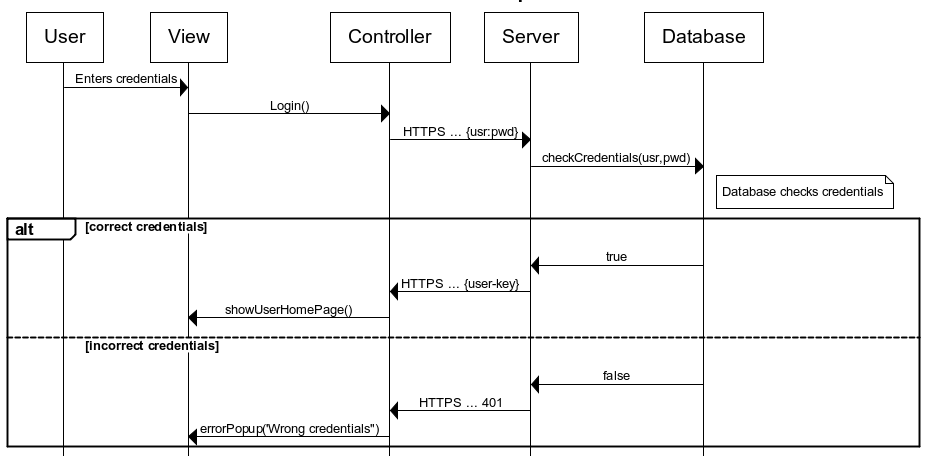
\includegraphics[width=145mm]{login-sequence.png}
 \caption{Vereenvoudigd sequentiediagram bij het inloggen}
 \label{login-sequence}
\end{figure}

\paragraph{Opmerking}

Bovenstaand sequentiediagram is slechts een vereenvoudiging van wat er in werkelijkheid gebeurt, zo zijn bijvoorbeeld procedures zoals checkCredentials in werkelijkheid asynchroon, en zullen ze dus geen boolean teruggeven, maar werken ze met callbacks.

Deze opmerking geldt ook voor alle andere sequentiediagrammen in dit onderdeel.

\subsection{Registreren}

Om een nieuwe gebruiker te registeren, dient men eerst een registratieformulier in te vullen. Om de gebruikerservaring hierbij de verbeteren zal dit gebeuren met real-time client-side validation (naast de server-side validation, die noodzakelijk is). 

Van zodra alle informatie is ingevuld, zal de client een identificatiestring terugkrijgen indien de nieuwe gebruiker succesvol is toegevoegd. Zoniet, zal de server een HTTP 40x-error teruggeven.

\begin{figure}[!h]
\centering
 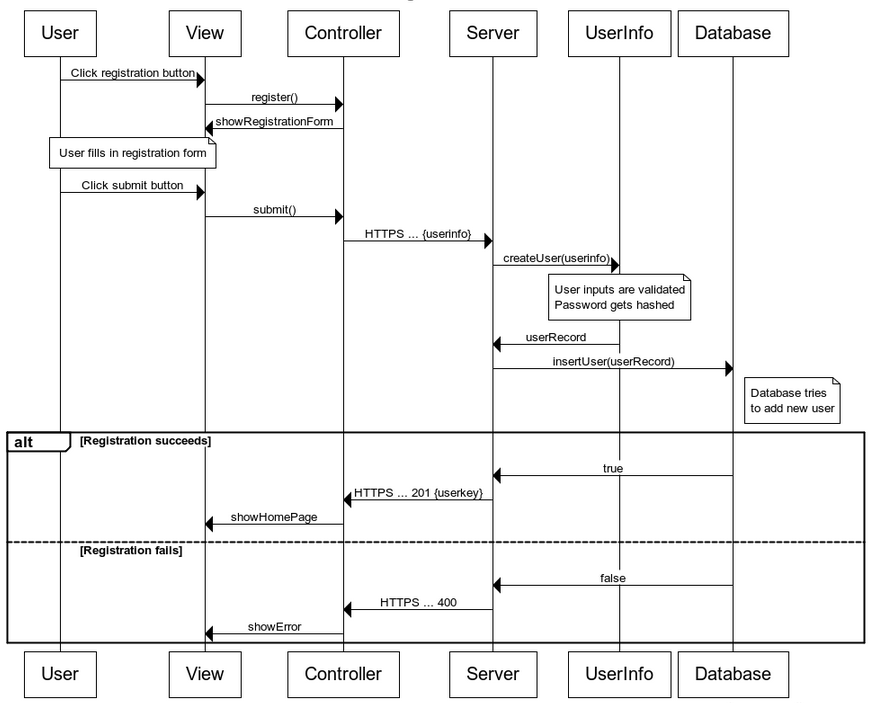
\includegraphics[width=145mm]{registration-sequence.png}
 \caption{Vereenvoudigd sequentiediagram bij het registreren}
 \label{register-sequence}
\end{figure}

\clearpage

\section{Human Interface Design}

\subsection{Filosofie}

Het front-end team van SKRIBL heeft een duidelijke visie over de uiteindelijke gebruikerservaring. Zo zal worden ingezet op een flat, anti-skeumorphistisch ontwerp dat futuristisch oogt. Daarnaast zullen ook de principes van `interfaceless interface' en de `three-click rule' worden gevolgd en zal gewerkt worden met vectori\"ele graphics in plaats van bitmaps.

\subsection{Overzicht}

Aangezien in de eerste sprint enkel inloggen en registreren werden ge\"implementeerd, is de functionaliteit van de grafische interface momenteel vrij beperkt. 

Hieronder vindt men de voorlopige functionaliteit van de UI:

\begin{description}

\item[Inloggen] Op de startpagina zal de gebruiker twee inputvelden terugvinden om zijn/haar naam en wachtwoord (niet textueel zichtbaar) in te geven. Daarna dient men enkel op de knop `inloggen' te klikken en zal bij een correct wachtwoord het dashboard van de gebruiker worden weergegeven, bij een incorrect wachtwoorden zal slechts een foutmelding worden getoond.

\item[Dashboard] Het dashboard is de startpagina van de gebruiker vanwaar men een overzicht kan krijgen van de meest relevante informatie voor de gebruiker (zoals recente publicaties). Momenteel is het enkel voorzien van een knop waarmee de gebruiker zich terug kan uitloggen.

\item[Registreren] Registratie gebeurt van zodra de gebruiker op de knop `registreren' klikt en het registratieformulier invult. Om de gebruikerservaring te verbeteren zal de client-side validatie real-time gebeuren en zal men pas op `submit' kunnen klikken van zodra alle informatie volledig en correct is ingevuld. Daarna komt de gebruiker ofwel terecht op zijn nieuw dashboard, ofwel krijgt hij een foutmelding te zien wanneer het toevoegen is mislukt.

\end{description}

\subsection{Screenshots}

\textit{[Momenteel heeft de front-end designer al verschillende ontwerpen voor de UI opgemaakt, maar is er in de groep nog geen consensus bereikt over de beste keuze hieruit. Van zodra dit het geval is, zal men in deze sectie screenshots van de GUI kunnen terugvinden.]}

\clearpage

\section{Externe API}

Naast de grafische interface, biedt het systeem ook een API aan voor externe ontwikkelaar die hun eigen applicaties willen integreren met SKRIBL. Dit gebeurt met RESTful API over HTTP. \\

\textit{[Het documenteren van deze API gebeurt normaal gezien automatisch aan de hand van Swagger. Aangezien deze momenteel echter nog niet is geconfigureerd en nog niet alle code is geschreven, volgt hieronder een (voorlopige) versie van de API.]} \\

\begin{description}
\item[POST /login] Deze request wordt gebruikt om in te loggen, men geeft gebruikersnaam en wachtwoord (over HTTPS) mee in JSON-formaat en krijgt een unieke identificatiestring terug van de server die men later moet meegeven bij bepaalde requests.

\item[GET /user/<username>] Op deze manier kan men in JSON-formaat relevante informatie van een bepaalde gebruiker in het systeem opvragen.

\item[PUT /user/<username>] Met deze request kan een nieuwe gebruiker op de server worden aangemaakt. Alle nodige gebruikersinformatie dient worden meegegeven bij de request als JSON-data.

\item[DELETE /user/<username>] Hierbij dient men expliciet zijn/haar identificatiestring mee te geven. Het resultaat is dat de aangeduide gebruiker uit het systeem zal worden verwijderd.

\end{description}

\clearpage

% \section{Requirements Matrix}

% Ten slotte kan men in onderstaande tabel terugvinden welke componenten verantwoordelijk % zijn voor welke opgestelde requirement. De codes die hierbij gebruikt worden voor de % requirements zijn afkomstig uit het SRS \cite{Xtreport:SRS}. De verschillende componenten % worden dan weer gerefereerd door hun nummering in sectie ... %insert reference.

%\begin{center}
%\begin{tabular}{|c|c|c|c|c|c|}
% \hline
% \textbf{Requirement} & View/Controller & 5.1 & 5.2 & 5.3 & 5.4 & 5.5\\
% \hline
% FR-U001              &                 &     &     &     &     &   \\
% FR-U002              &                 &     &     &     &     &   \\
% FR-U003              &                 &     &     &     &     &   \\
% FR-U004              &                 &     &     &     &     &   \\
% FR-U005              &                 &     &     &     &     &   \\
% FR-U006              &                 &     &     &     &     &   \\
% FR-U007              &                 &     &     &     &     &    \\
% FR-U008              &                 &     &     &     &     &    \\
% FR-U009              &                 &     &     &     &     &   \\
% FR-U010              &                 &     &     &     &     &   \\
% FR-U011              &                 &     &     &     &     &   \\
% FR-U012              &                 &     &     &     &     &   \\
% FR-U013              &                 &     &     &     &     &   \\
% FR-U014              &                 &     &     &     &     &   \\
% FR-U015              &                 &     &     &     &     &   \\
% FR-U016              &                 &     &     &     &     &   \\
% FR-U017              &                 &     &     &     &     &   \\
% FR-U018              &                 &     &     &     &     &   \\
% FR-U019              &                 &     &     &     &     &   \\
% FR-U020              &                 &     &     &     &     &   \\
% FR-U021              &                 &     &     &     &     &   \\
% FR-U022              &                 &     &     &     &     &   \\
% FR-U023              &                 &     &     &     &     &   \\
% FR-U024              &                 &     &     &     &     &   \\
% FR-U025              &                 &     &     &     &     &   \\
% FR-U026              &                 &     &     &     &     &   \\
% FR-U027              &                 &     &     &     &     &   \\
% \hline
% NFR-S001             &                 &     &     &     &     &   \\
% NFR-S002             &                 &     &     &     &     &   \\
% \hline
%\end{tabular}
%\end{center}

\end{document}
